%Created by Roland Pastorino in 2013
%Contact info: roland.pastorino@mech.kuleuven.be / www.rolandpastorino.com
%If you want to include your modifications in the template and make them available for everybody, you can contact the "KU Leuven, Dienst Communicatie, Afdeling Positionering en Marketing" (marketing@dcom.kuleuven.be) or myself.

\documentclass[11pt,t]{beamer}
\mode<presentation> {\usetheme{kuleuven}}

\usepackage[backend=biber]{biblatex}
\bibliography{bib.bib}
\setbeamertemplate{bibliography item}{}

\usepackage{rotating}
\usepackage{environ}
\NewEnviron{Answer}
{%
\noindent
\rotatebox[origin=c]{180}{%
\noindent
\begin{minipage}[t]{\linewidth}
\begin{answer}
\BODY
\end{answer}%
\end{minipage}%
}%
}%

%%%%%%%%%%%%%%%%%%%%%%%%%%%%%%%%%%%%%%%%
%info
\title{Privacy-friendly machine learning algorithms for intrusion detection systems}
\author{Henri De Plaen}
\institute{Master Applied Mathematics, KU Leuven}
\subtitle{Supervisor: Pr. dr. ir. Bart Preneel}
\date{December 22, 2017 Leuven, Belgium}
%pdf metadata
	\subject{KU Leuven}
	\keywords{KU Leuven}
\graphicspath{{graphics/}} % path to the graphics folder
%%%%%%%%%%%%%%%%%%%%%%%%%%%%%%%%%%%%%%%%
\begin{document}
%title page
	\setbeamertemplate{headline}[title_page]
	\setbeamertemplate{footline}[title_page]
	\csname beamer@calculateheadfoot\endcsname %recalculate head and foot dimension
		\begin{frame}
			\titlepage
		\end{frame}
%head and foot for body text	
	\setbeamertemplate{headline}[body]
	\setbeamertemplate{footline}[body]

%%%%%%%%%%%%%%%%%%%%%%%%%%%%%%%%%%%%%%%%%%
\begin{frame}{Outline}
	\vskip 5mm
	\hfill	{\large \parbox{1\textwidth}{\tableofcontents[hideallsubsections]}}
\end{frame}

%%%%%%%%%%%%%%%%%%%%%%%%%%%%%%%%%%%%%%%%
\section{Introduction}
%--------------------------------------
\begin{frame}{General context}
\begin{column}{.7\textwidth}
\begin{itemize}
    \item As computers are used more and more (including for sensible data), and the connection between them increases as well, there is a constant need for better intrusion detection systems.
    \item Machine learning algorithms can increase performance of a lot of existing applications, but they need a significant dataset.
    \item The amount of data increases as well, but remains sensible in the case of intrusion detection systems, hence the need for encryption.
\end{itemize}
	\end{column}
\begin{column}{.3\textwidth}
		\centering
		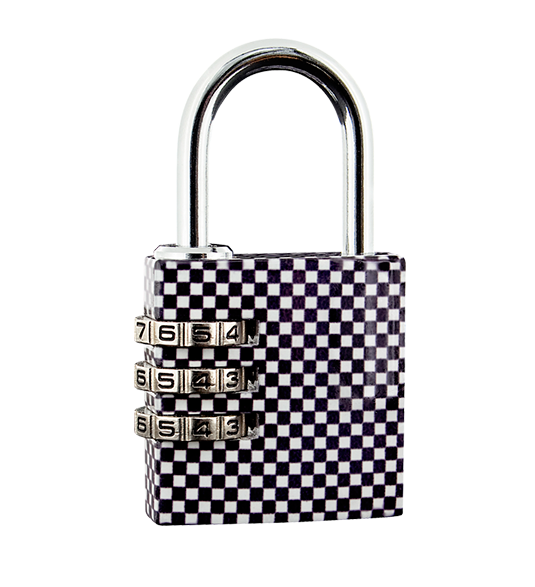
\includegraphics[width=1\textwidth]{cadenas}
	\end{column}
\end{frame}
%--------------------------------------
\begin{frame}[plain,c]{Problem statement (attempt I)}
\begin{center}
\begin{quote}
    Privacy-friendly data pooling for enhancing intrusion detection systems
\end{quote}
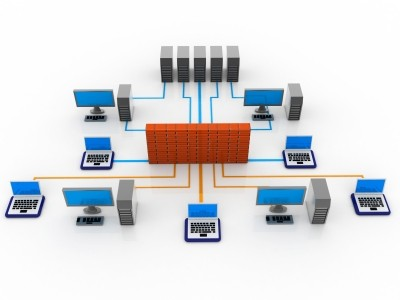
\includegraphics[width=.6\textwidth]{nids}
\end{center}
\end{frame}
%%%%%%%%%%%%%%%%%%%%%%%%%%%%%%%%%%%%%%%
\section{Intrusion detection systems}
%--------------------------------------
\begin{frame}{Introduction}
Different types, based on where the intrusion takes place
\begin{itemize}
    \item Network Intrusion Detection System (NIDS)
    \item Host Intrusion Detection System (HIDS)
    \item Hybrid Intrusion Detection System
\end{itemize}
\vfill
Different detection methods
\begin{itemize}
    \item Signature based
    \begin{itemize}
        \item Advantages: accuracy and time
        \item Disadvantages: only known intrusion types are detected
    \end{itemize}
    \item Anomaly based
    \begin{itemize}
        \item Advantages: new intrusion types can be detected
        \item Disadvantages: malicious activity disguised as normal traffic can pass through
    \end{itemize}
    \item Machine learning (classification)
\end{itemize}
\end{frame}
%--------------------------------------
\begin{frame}{Applying big scale machine learning}
Different types, based on where the intrusion takes place
\begin{itemize}
    \item Network Intrusion Detection System (NIDS)
    \begin{itemize}
        \item Advantages: detects attack before it occurs
        \item Disadvantages: needs to be implemented on the network
    \end{itemize}
    \item Host Intrusion Detection System (HIDS)
    \begin{itemize}
        \item Advantages: collects broader data type
        \item Disadvantages: needs to be implemented on each machine and only detects after the intrusion
    \end{itemize}
    \item Hybrid Intrusion Detection System
    \begin{itemize}
        \item Advantages: much more effective
        \item Disadvantages: huge implementation necessary, not privacy-friendly
    \end{itemize}
\end{itemize}
\end{frame}
%--------------------------------------
\begin{frame}[plain,c]{Problem statement (attempt II)}
\begin{center}
    \begin{quote}
    Privacy-friendly data pooling for machine learning network intrusion detection system
\end{quote}
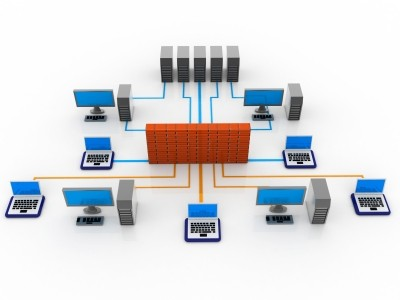
\includegraphics[width=.6\textwidth]{nids}
\end{center}
\end{frame}
%%%%%%%%%%%%%%%%%%%%%%%%%%%%%%%%%%%%%%%
\section{Multiparty computation}
%--------------------------------------
\begin{frame}{Introduction: example (1)}
Addition over $\mathbb{Z}_2$
\begin{itemize}
    \item $i$ players have each a secret number $n_i$
    \item they want to know if the sum of their numbers is even or uneven. $\Sigma n_i \mod 2 =0$ or $1$ ?
    \item they don't want anybody except them to know their number
\end{itemize}
\vfill

Solution
\begin{itemize}
    \item each players divides its number $n_i$ into $j$ $m_{i,j}$ parts. $\Sigma m_{i,j} = n_i$
    \item $j$ players each receive the $m_{i,j}$-part of each $i$ players, sums it up and say if it is even or not. $\Sigma_i m_{i,j} \mod 2 = 0$ or $1$.
    \item the results of all $j$ players is then summed up and is even if $\Sigma n_i \mod 2 =0$ and uneven otherwise. The problem is resolved.
\end{itemize}

\end{frame}
%--------------------------------------
\begin{frame}{Introduction: example (2)}
\begin{center}
	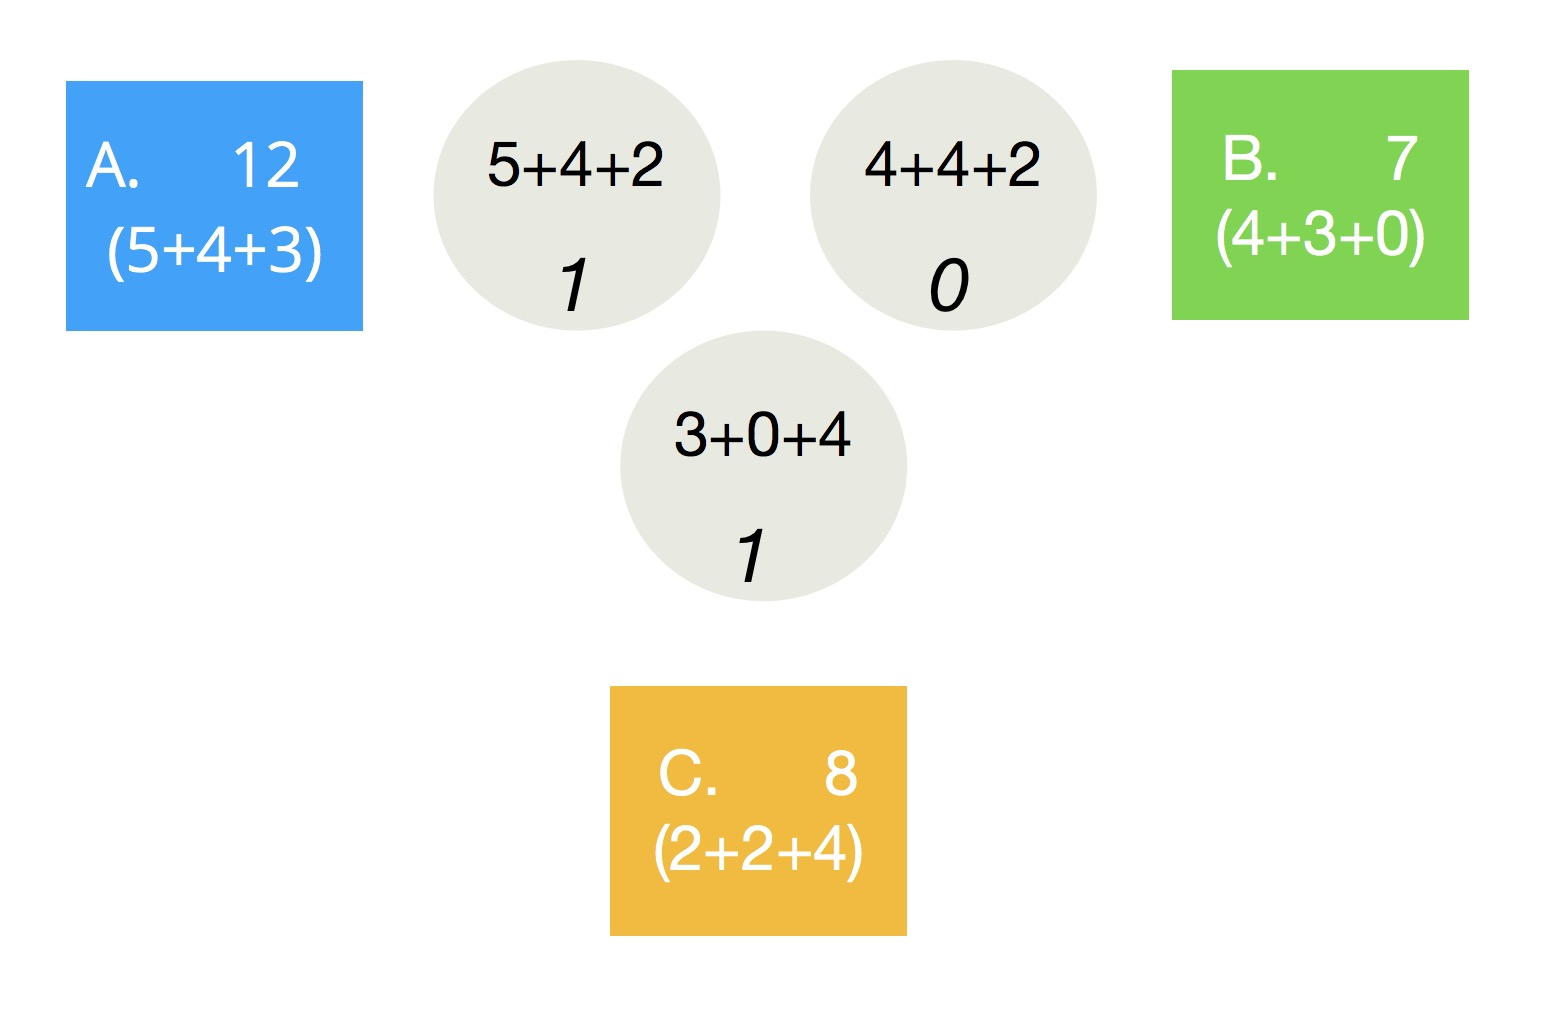
\includegraphics[width=\textwidth]{mpc}
\end{center}
\end{frame}
%--------------------------------------
\begin{frame}{Two types of circuits}
Garbled
\begin{itemize}
    \item Boolean circuit
    \item Based on OT
    \item Constant number of rounds
\end{itemize}
Arithmetic
\begin{itemize}
    \item Based on somewhat homomorphic encryption (SHE)
    \item Allows for addition and multiplication
\end{itemize}
\begin{center}
	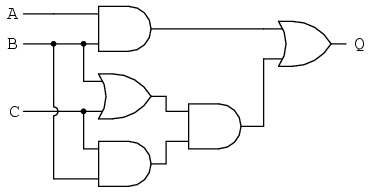
\includegraphics[width=.4\textwidth]{boolean}
\end{center}
\end{frame}
%--------------------------------------
\begin{frame}{Oblivious Transfer}
\begin{itemize}
    \item The receiver doesn't get any information on the strings he didn't recieve
    \item The sender doesn't know which string was asked
\end{itemize}
\begin{center}
	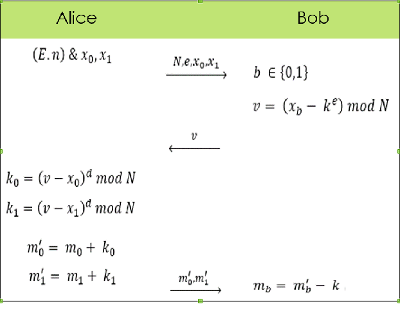
\includegraphics[width=.5\textwidth]{oblivious}
\end{center}
\end{frame}
%--------------------------------------
\begin{frame}{Garbled circuits}
\begin{center}
	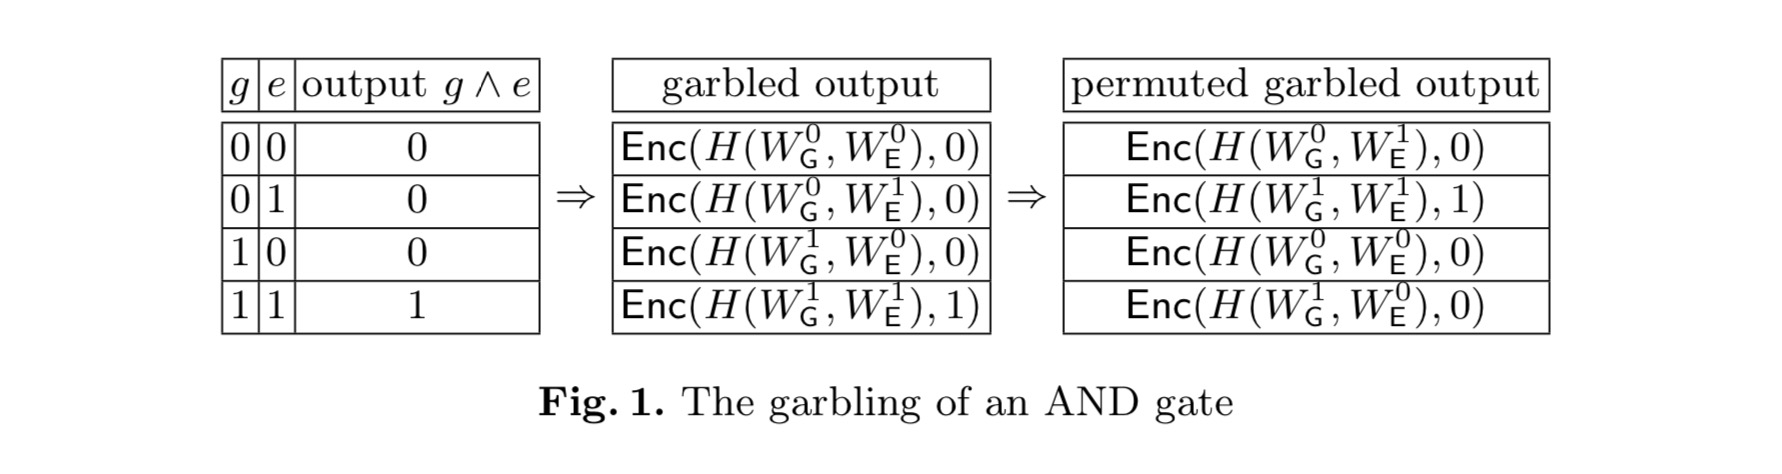
\includegraphics[width=\textwidth]{garbled}
\end{center}
\end{frame}
%--------------------------------------
\begin{frame}{Intrusion detection systems}
Different leads
\begin{itemize}
    \item Fairplay (boolean, n-party)
    \item BMR (boolean, n-party)
    \item Sharemind (3-party, proprietary)
    \item VIFF (obsolete)
    \item ABY (2-party)
    \item \bf{SPDZ} (artihmetic, n-party)
\end{itemize}
\end{frame}
%--------------------------------------
\begin{frame}[plain,c]{Problem statement (attempt III)}
\begin{center}
\begin{quote}
    Privacy-friendly collaborative network intrusion detection system
\end{quote}
	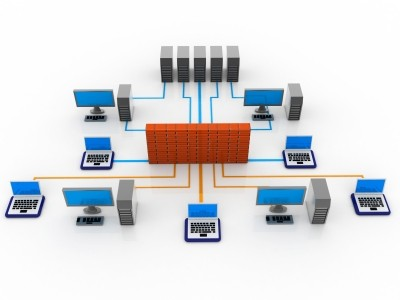
\includegraphics[width=.6\textwidth]{nids}
\end{center}
\end{frame}
%%%%%%%%%%%%%%%%%%%%%%%%%%%%%%%%%%%%%%%
\section{Methodology}
%--------------------------------------
\begin{frame}{Benchmarking}
\begin{column}{.5\textwidth}
Datasets
\begin{itemize}
    \item KDD CUP '99
    \item AWID
    \item PCAP
    \item UNB ISCX
    \item CSIC 2010 HTTP Dataset
    \item West Point - NSA DataSet
\end{itemize}
	\end{column}
\begin{column}{.5\textwidth}
		\centering
		
\includegraphics[width=.8\textwidth]{datasets}
	\end{column}
\end{frame}
%--------------------------------------
\begin{frame}{Design}
\begin{column}{.5\textwidth}
		\centering
		
\includegraphics[width=.8\textwidth]{nn}
	\end{column}
\begin{column}{.5\textwidth}
Current research algorithms
\begin{itemize}
    \item Semi-supervised learning algorithms with fuzziness
    \item K-Nearest Neighbors
    \item Support Vector Machines
    \item Bayes Classifier
    \item EM-Clustering
    \item Genetic algorithms
    \item Classification Tree
\end{itemize}
	\end{column}

\end{frame}
%--------------------------------------
\begin{frame}{Prototyping}
\begin{itemize}
    \item Build on existing application (e.g. Bro Network Security Monitor, OpenNMS,...), in the form of a plug-in.
    \item Feed with constant new data, provided from other analysis tools
    \item User-friendly
    \item Off-line
\end{itemize}
\begin{center}
    
\includegraphics[width=.2\textwidth]{plugin}
\end{center}
\end{frame}
%--------------------------------------
\begin{frame}{Agenda}
\begin{center}
    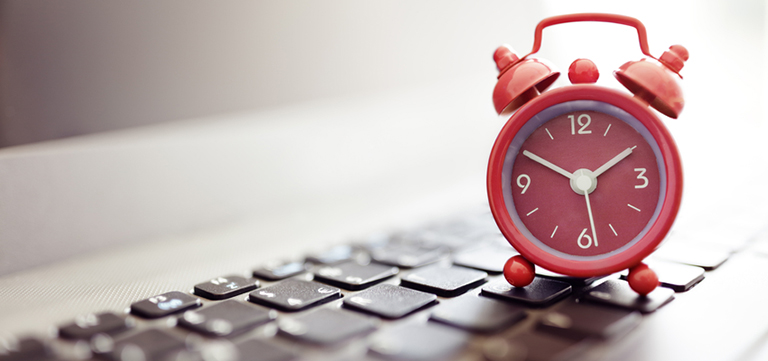
\includegraphics[width=.5\textwidth]{deadlines}
\end{center}
\begin{itemize}
    \item Begin March: Benchmark and designing working machine-learning algorithm
    \item Begin April: Design of final algorithm including MPC
    \item Begin May: Prototyping as a plug-in
    \item Begin June: Poster and report
\end{itemize}
\end{frame}
%%%%%%%%%%%%%%%%%%%%%%%%%%%%%%%%%%%%%%%
\section{Conclusion}
%--------------------------------------
\begin{frame}{References}
\begin{center}
    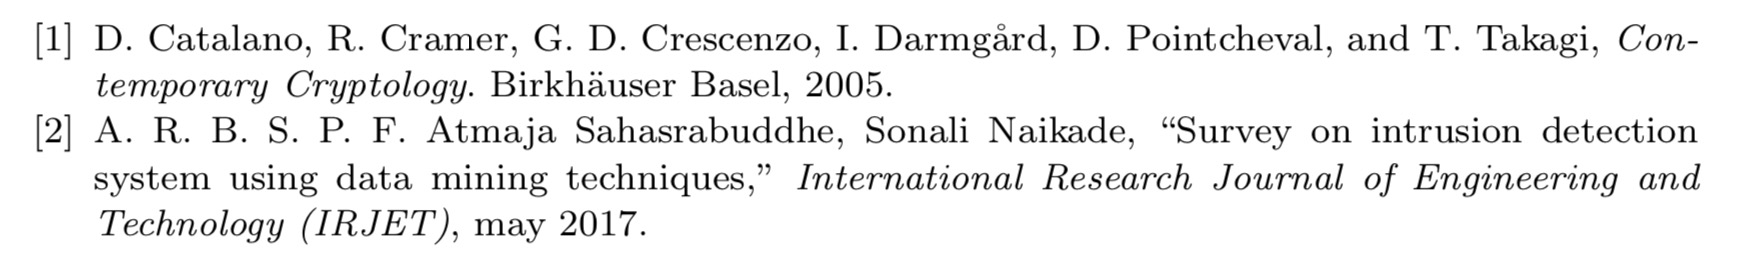
\includegraphics[width=\textwidth]{bib}
\end{center}
\end{frame}
%--------------------------------------
\begin{frame}{Conclusion}
Further optimizations
\begin{itemize}
    \item Hybrid Intrusion Detection Systems
    \item Speed and complexity optimizations (research on HE)
    \item Deep learning
\end{itemize}
\begin{center}
    
\includegraphics[width=.5\textwidth]{thankyou}
\end{center}
\end{frame}
%--------------------------------------
\begin{frame}
\frametitle{Questions?}
\begin{center}
    
\includegraphics[width=\textwidth,height=0.8\textheight,keepaspectratio]{graphics/questions.jpg}
\end{center}
\end{frame}
\end{document}